\chapter{Literature Review}
\label{chap:literature-review}

\section{Chapter Overview}

This chapter establishes the technical and musical context for modelling the Boss DS-1 as a nonlinear audio system, tracing the path from established virtual analog approaches to data-driven neural modelling. It explains why recurrent architectures suit distortion circuits with memory-dependent behaviour and positions the research gap behind the GRU versus LSTM comparison at the heart of this project.

\section{Analog Distortion}

Digitally emulating analog audio hardware, a discipline known as virtual analog (VA) modelling, has persisted because listeners keep reaching for the sonic character of classic equipment. Terms like ``warmth'', ``richness'', ``character'', and ``organic feel'' are vague, but they all point to the audible result of nonlinear electronic components pushed near or beyond their intended linear regions. When an audio signal passes through a vacuum tube, transistor, or diode operating in that region, the device introduces new frequency content not present in the original signal: \textbf{harmonic distortion}.

None of this was planned. The sound that became a cornerstone of modern guitar music grew out of the limitations and outright failures of early amplification technology. Its origins are usually traced to the 1950s, when musicians discovered that overdriving amplifiers produced an unintentionally powerful, buzzing quality. The 1951 recording of \textit{Rocket 88} is often cited here: a damaged speaker cone produced a distorted tone that ended up defining the record's character, and musicians quickly started chasing that quality deliberately, even damaging their own equipment to get it.

The commercialization of this effect in the 1960s was marked by the Gibson Maestro FZ-1 Fuzz-Tone, shown in Figure~\ref{fig:maestro-fz1}. Its association with The Rolling Stones made clear that distortion was a controllable musical effect, not a technical fault, and manufacturers followed with a wide range of devices that would come to define the sound of rock, punk, metal, and alternative music for decades.

\begin{figure}[htbp]
    \centering
    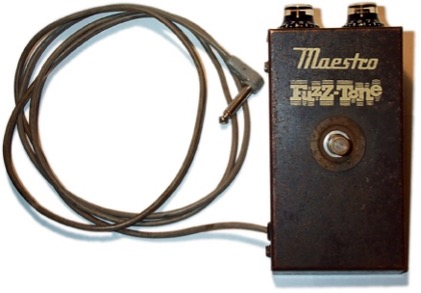
\includegraphics[width=0.5\textwidth]{images/maestro_fz1.jpg}
    \caption[Gibson Maestro FZ-1 Fuzz-Tone pedal]{Gibson Maestro FZ-1 Fuzz-Tone pedal. Image source: \cite{wikipedia_maestro_fz1_2026}.}
    \label{fig:maestro-fz1}
\end{figure}

The specific character of a distortion effect is determined by the blend of harmonics it generates, which is dictated by the circuit topology. Two broad categories are useful here:

\begin{itemize}
    \item \textbf{Even-order harmonics} are integer multiples such as two, four, and six times the fundamental frequency. They are generally perceived as musically consonant and can add smoothness and constructive brightness. The asymmetrical clipping introduced by a single-ended transistor stage, for example, can produce even-order harmonics.
    \item \textbf{Odd-order harmonics} are integer multiples such as three, five, and seven times the fundamental frequency. They tend to sound harsher or grittier, contributing to the richness and depth of many distortion sounds. The symmetric clipping of back-to-back diodes is a common design that mainly generates odd-order harmonics.
\end{itemize}

Beyond simple harmonic generation, the perceived warmth of analog equipment also comes from subtler imperfections: transformer hysteresis, dynamic compression, circuit sag under heavy load. Getting all of this right in the digital domain has proven genuinely difficult.

\section{The Boss DS-1 as a Modelling Target}

This dissertation focuses on the Boss DS-1, shown in Figure~\ref{fig:boss-ds1-pedal}. Released in 1978, it is a widely used distortion pedal whose circuit combines several gain, clipping, and filtering stages into a recognisable high-gain guitar sound.

\begin{figure}[htbp]
    \centering
    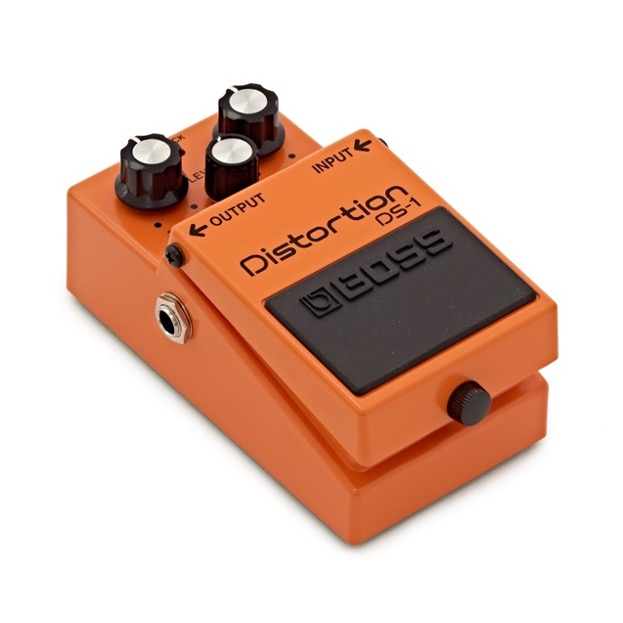
\includegraphics[width=0.55\textwidth]{images/boss_ds1_pedal.jpg}
    \caption[Boss DS-1 distortion pedal]{Boss DS-1 distortion pedal. Image source: \cite{boss_ds1_product_2026}.}
    \label{fig:boss-ds1-pedal}
\end{figure}

The DS-1 circuit, shown in Figure~\ref{fig:boss-ds1-circuit}, breaks down into four main stages:

\begin{figure}[htbp]
    \centering
    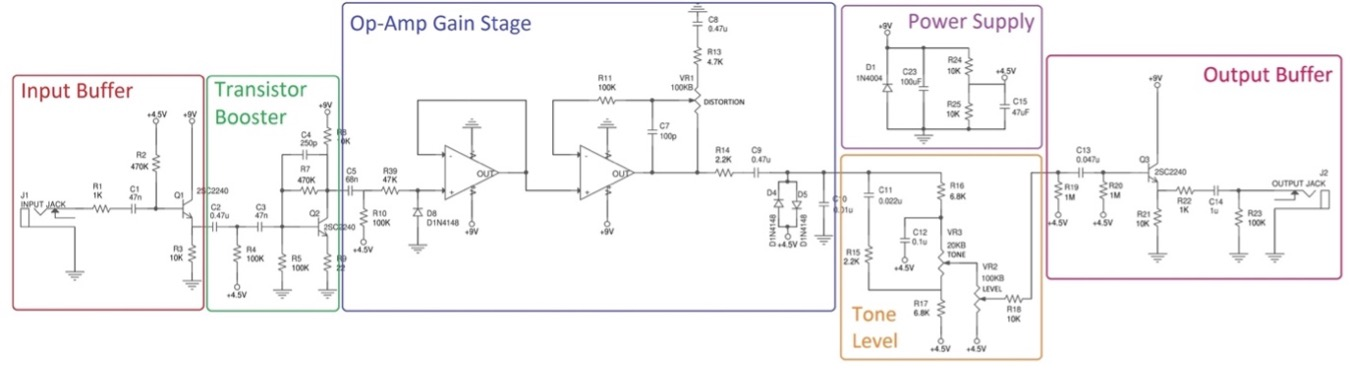
\includegraphics[width=0.9\textwidth]{images/boss_ds1_circuit.jpg}
    \caption[Boss DS-1 circuit used as the modelling target]{Boss DS-1 circuit used as the modelling target. Diagram source: \cite{noauthor_electrosmash_nodate}.}
    \label{fig:boss-ds1-circuit}
\end{figure}

\begin{enumerate}
    \item \textbf{Input buffer stage}: an emitter-follower transistor stage that provides high input impedance and helps preserve the guitar's signal before further processing.

    \item \textbf{Transistor booster stage}: a gain stage with pre-clipping high-pass filtering that tightens the low end and can introduce some asymmetrical soft clipping.

    \item \textbf{Op-amp gain and hard-clipping stage}: the main distortion stage, where variable op-amp gain drives anti-parallel silicon diodes that produce the DS-1's characteristic hard-clipped sound.

    \item \textbf{Tone and level stage}: a passive tone circuit and output stage that reshape the clipped signal, including the familiar mid-scooped balance associated with the pedal.
\end{enumerate}


\section{Virtual Analog Modelling Approaches}

\subsection{White-Box Circuit Modelling}

Virtual analog modelling has historically split into two broad paradigms: white-box and black-box. The distinction is one of philosophy as much as technique, and each approach carries real trade-offs between accuracy, interpretability, and computational cost.

White-box, or physical, modelling starts from the premise that a sufficiently complete mathematical description of a circuit can be solved digitally to reproduce its output. The process begins with a detailed circuit schematic; using Kirchhoff's current and voltage laws, the circuit is translated into a system of nonlinear \textbf{ordinary differential equations (ODEs)}. Software such as \textbf{SPICE} automates this step using Modified Nodal Analysis (MNA). Other white-box techniques include Wave Digital Filters (WDFs) and state-space models, each offering a different formalism for the same goal.

White-box modelling's appeal is interpretability: a good circuit model can, in principle, explain the contribution of each component and reproduce the device across a wide range of conditions. For real-time audio, though, two practical problems arise.

First, the computational cost can be prohibitive. Distortion circuits contain nonlinear elements, so their systems of equations cannot generally be solved in closed form at each sample. An iterative numerical method such as Newton--Raphson iteration is needed to converge on a solution, and running that at every sample is expensive; the sequential nature of the computation also resists parallelization. A detailed SPICE simulation can easily run far slower than real time.

Second, the approach depends on detailed and accurate knowledge of the circuit. The simulation is only as good as the component models and parameter values supplied to it. Real components vary across manufacturing tolerances and age, so a model built on ideal datasheet values may behave quite differently from a specific physical unit, and characterizing those individual imperfections is rarely practical.

\subsection{Traditional Black-Box and Signal Processing Methods}

Black-box modelling treats the device as an input-output system rather than deriving full circuit equations. For a guitar pedal, the dry signal becomes the input and the recorded pedal output becomes the target, avoiding many of the practical burdens of white-box modelling \cite{martinez_ramirez_deep_2020,wright_real-time_2019}.

The simplest version is static waveshaping, often combined with filters before and after the nonlinearity. Yeh et al. describe this as a computationally efficient filter--distortion--filter simplification of analog pedal behaviour \cite{yeh_simplified_2007}. The problem is that it is memoryless: real pedals such as the DS-1 respond to recent signal history, not just the current sample.

Linear convolution works well for linear time-invariant systems such as cabinets and EQ curves, but not for a nonlinear distortion pedal. More expressive block-oriented models, including Wiener, Hammerstein, and Wiener--Hammerstein structures, combine filters and nonlinearities more flexibly, but still assume a simplified signal path \cite{wright_real-time_2019}. A pedal with the DS-1's interacting gain, filtering, clipping, and tone stages pushes beyond what these structures handle cleanly.

\section{Deep Learning for Nonlinear Audio Systems}

Deep learning extends black-box modelling by replacing a hand-designed structure with a trainable function learned from paired recordings. Here, the dry guitar signal is the input and the Boss DS-1 recording is the target. The model receives no explicit circuit description; it learns the input-to-output mapping directly from data. Martínez Ramírez et al. describe this as an end-to-end black-box strategy that reduces the need for detailed prior knowledge of the processor being modelled \cite{martinez_ramirez_deep_2020}. The tradeoff is interpretability: a learned function is harder to inspect than a circuit simulation.

Damskägg et al. showed that WaveNet-style models can emulate distortion pedals including the DS-1 in real time, while Wright et al. showed that compact recurrent models can achieve strong accuracy at lower cost than larger convolutional systems \cite{wright_real-time_2019}. Practical tools such as GuitarLSTM and SmartGuitarAmp further demonstrate a viable path from Python training to JUCE-based deployment \cite{GuitarML_GuitarLSTM,GuitarML_SmartGuitarAmp}.

\section{Sequence Modelling and Recurrent Neural Networks for Audio Emulation}

Audio is a time sequence, so nonlinear systems with memory cannot be described only by instantaneous sample values. Circuits containing filters and reactive components respond to recent signal history as well as the current input, which makes sequence modelling especially relevant for distortion emulation.

Recurrent neural networks are designed for this problem. They process one time step at a time while maintaining an internal state, so the predicted output depends on the current input, previous state, and learned parameters \cite{wright_real-time_2019}. For a distortion pedal, that hidden state may encode recent level, envelope, or spectral context.

For plugin deployment, RNNs have a practical advantage: they are naturally causal and can process audio sample by sample without look-ahead, as long as the hidden state is preserved across audio blocks. Training is harder than for feedforward networks, and is typically handled with segmented audio and truncated back-propagation through time.

\section{LSTM and GRU Architectures}

Basic recurrent networks can be difficult to train over longer sequences. LSTM and GRU architectures address this with learned gates that control what information is retained, updated, or discarded.

\subsection{Long Short-Term Memory}

The Long Short-Term Memory architecture was introduced to improve how recurrent networks preserve information over time \cite{hochreiter_long_1997}. Its gated hidden and cell-state structure suits nonlinear audio tasks involving filtering, envelope dependence, and level-dependent behaviour. Wright et al. reported strong LSTM performance in real-time black-box modelling, and Cassidy and De Sena used an LSTM-RNN in perceptual evaluation of high-gain amplifier models \cite{wright_real-time_2019,cassidy_perceptual_2023}. The cost, literally, is higher: for the same hidden size, an LSTM typically requires more parameters and compute than a GRU.

\subsection{Gated Recurrent Unit}

The Gated Recurrent Unit is a simpler gated recurrent architecture \cite{cho_learning_2014}. Because it uses fewer gates than an LSTM, a GRU with the same hidden size usually has fewer parameters and lower computational cost, though it may have less flexibility in how it regulates temporal information.

The relevant question for this project is not which architecture is universally better, but which gives the best accuracy-to-efficiency balance on this specific DS-1 task.

\section{Real-Time Deployment and Neural Inference}

Training can happen in Python, but a DAW plugin must load the trained model and run forward inference in C++. That shift from research environment to real-time system introduces hard constraints.

Real-time audio threads must avoid blocking operations: allocation, file access, locks. Chowdhury presents RTNeural as a lightweight C++ inference library for hard real-time systems, making it directly relevant to the JUCE-based plugin workflow used here \cite{chowdhury_rtneural_2021}.

Deployment constraints also feed back into architectural choice. A model that performs well offline but cannot run cleanly in a plugin does not fully answer the research question. A slightly less accurate model that works reliably in real time may simply be more useful.

\section{Evaluation of Neural Audio Models}

The primary metric in this project is Error-to-Signal Ratio (ESR), which compares prediction-error energy with target-signal energy rather than treating error in purely absolute terms.

ESR is widely used in neural virtual analog work, and some training pipelines pair it with pre-emphasis so that the loss pays more attention to high-frequency content important to distortion \cite{wright_real-time_2019,cassidy_perceptual_2023}. A DC term is also useful because a learned offset can reduce headroom and indicate low-frequency bias \cite{wright_real-time_2019}.

Lower ESR does not automatically mean that listeners will hear the model as more accurate or prefer it. Stronger perceptual claims would require formal listening tests such as ABX or MUSHRA-style evaluation \cite{ITU_BS1534_3,cassidy_perceptual_2023}.

\section{Research Gap and Positioning of This Study}

White-box methods offer interpretability but require detailed circuit knowledge and can be computationally expensive. Black-box methods sidestep that requirement but typically rely on simplifying assumptions about signal flow. Deep neural networks learned from paired recordings offer a more flexible data-driven path \cite{yeh_simplified_2007,martinez_ramirez_deep_2020}.

There are useful precedents in the neural virtual analog literature. Damskägg et al. demonstrated real-time WaveNet-style modelling of pedals including the DS-1, Wright et al. showed that compact recurrent networks can model nonlinear audio devices efficiently, and Martínez Ramírez et al. situated these developments within a broader deep-learning audio-effects framework \cite{wright_real-time_2019,martinez_ramirez_deep_2020}. Cassidy and De Sena further show that objective accuracy should be considered alongside perceptual questions \cite{cassidy_perceptual_2023}.

What is missing from the literature is a controlled GRU versus LSTM comparison on a single physical device under matched recording, training, evaluation, and deployment conditions. This project does not contribute a new architecture; it contributes a documented end-to-end workflow built around that focused question: a matched dry/wet dataset, trained models, exported JSON weights, and a JUCE/RTNeural plugin \cite{candy_practice-based_2018,batty_research_2024}.
